%   Copyright 2012 Comet Engineering, Patrick Haring & Christian Bürgi
%
%   Licensed under the Apache License, Version 2.0 (the "License");
%   you may not use this file except in compliance with the License.
%   You may obtain a copy of the License at
%
%       http://www.apache.org/licenses/LICENSE-2.0
%
%   Unless required by applicable law or agreed to in writing, software
%   distributed under the License is distributed on an "AS IS" BASIS,
%   WITHOUT WARRANTIES OR CONDITIONS OF ANY KIND, either express or implied.
%   See the License for the specific language governing permissions and
%   limitations under the License.

\documentclass[fontsize=12pt,
               paper=a4,
               twoside=false,
               parskip=half,
               ]{scrartcl}

% Load the packages
%   Copyright 2012 Comet Engineering, Patrick Haring & Christian Bürgi
%
%   Licensed under the Apache License, Version 2.0 (the "License");
%   you may not use this file except in compliance with the License.
%   You may obtain a copy of the License at
%
%       http://www.apache.org/licenses/LICENSE-2.0
%
%   Unless required by applicable law or agreed to in writing, software
%   distributed under the License is distributed on an "AS IS" BASIS,
%   WITHOUT WARRANTIES OR CONDITIONS OF ANY KIND, either express or implied.
%   See the License for the specific language governing permissions and
%   limitations under the License.

% Packages Template
% =================
% 
% Contains packages used for project documentation
% 
% @author burgc5
% 
% To use this simply enter: %   Copyright 2012 Comet Engineering, Patrick Haring & Christian Bürgi
%
%   Licensed under the Apache License, Version 2.0 (the "License");
%   you may not use this file except in compliance with the License.
%   You may obtain a copy of the License at
%
%       http://www.apache.org/licenses/LICENSE-2.0
%
%   Unless required by applicable law or agreed to in writing, software
%   distributed under the License is distributed on an "AS IS" BASIS,
%   WITHOUT WARRANTIES OR CONDITIONS OF ANY KIND, either express or implied.
%   See the License for the specific language governing permissions and
%   limitations under the License.

% Packages Template
% =================
% 
% Contains packages used for project documentation
% 
% @author burgc5
% 
% To use this simply enter: %   Copyright 2012 Comet Engineering, Patrick Haring & Christian Bürgi
%
%   Licensed under the Apache License, Version 2.0 (the "License");
%   you may not use this file except in compliance with the License.
%   You may obtain a copy of the License at
%
%       http://www.apache.org/licenses/LICENSE-2.0
%
%   Unless required by applicable law or agreed to in writing, software
%   distributed under the License is distributed on an "AS IS" BASIS,
%   WITHOUT WARRANTIES OR CONDITIONS OF ANY KIND, either express or implied.
%   See the License for the specific language governing permissions and
%   limitations under the License.

% Packages Template
% =================
% 
% Contains packages used for project documentation
% 
% @author burgc5
% 
% To use this simply enter: \input{./packages.tex}

\usepackage[utf8]{inputenc}
\usepackage[T1]{fontenc}

% Set font to latin modern
\usepackage{lmodern}

\usepackage[pdftex]{graphicx}
\usepackage{epstopdf}

% Create links in pdf documents
\usepackage[colorlinks,pdfpagelabels,pdfstartview=FitH,bookmarksopen=true,bookmarksnumbered=true,linkcolor=black,plainpages=false,hypertexnames=false,citecolor=black] {hyperref}
\hypersetup{
    colorlinks,%
    citecolor=black,%
    filecolor=black,%
    linkcolor=black,%
    urlcolor=black
}
\urlstyle{same}

% Use \enquote{} to create quotation marks
\usepackage{csquotes}

% Create professional tables with booktabs
% @see http://en.wikibooks.org/wiki/LaTeX/Tables#Professional_tables
\usepackage{booktabs}

% Customizable enumerates/itemizes
\usepackage{enumitem}

% git meta information
\usepackage{gitinfo}


\usepackage[utf8]{inputenc}
\usepackage[T1]{fontenc}

% Set font to latin modern
\usepackage{lmodern}

\usepackage[pdftex]{graphicx}
\usepackage{epstopdf}

% Create links in pdf documents
\usepackage[colorlinks,pdfpagelabels,pdfstartview=FitH,bookmarksopen=true,bookmarksnumbered=true,linkcolor=black,plainpages=false,hypertexnames=false,citecolor=black] {hyperref}
\hypersetup{
    colorlinks,%
    citecolor=black,%
    filecolor=black,%
    linkcolor=black,%
    urlcolor=black
}
\urlstyle{same}

% Use \enquote{} to create quotation marks
\usepackage{csquotes}

% Create professional tables with booktabs
% @see http://en.wikibooks.org/wiki/LaTeX/Tables#Professional_tables
\usepackage{booktabs}

% Customizable enumerates/itemizes
\usepackage{enumitem}

% git meta information
\usepackage{gitinfo}


\usepackage[utf8]{inputenc}
\usepackage[T1]{fontenc}

% Set font to latin modern
\usepackage{lmodern}

\usepackage[pdftex]{graphicx}
\usepackage{epstopdf}

% Create links in pdf documents
\usepackage[colorlinks,pdfpagelabels,pdfstartview=FitH,bookmarksopen=true,bookmarksnumbered=true,linkcolor=black,plainpages=false,hypertexnames=false,citecolor=black] {hyperref}
\hypersetup{
    colorlinks,%
    citecolor=black,%
    filecolor=black,%
    linkcolor=black,%
    urlcolor=black
}
\urlstyle{same}

% Use \enquote{} to create quotation marks
\usepackage{csquotes}

% Create professional tables with booktabs
% @see http://en.wikibooks.org/wiki/LaTeX/Tables#Professional_tables
\usepackage{booktabs}

% Customizable enumerates/itemizes
\usepackage{enumitem}

% git meta information
\usepackage{gitinfo}



\begin{document}

% Document title for title.tex
\newcommand{\doctitle}{Game manual}
% Titlepage Template
% ==================
% 
% @author burgc5
% 
% To use this simply enter: % Titlepage Template
% ==================
% 
% @author burgc5
% 
% To use this simply enter: % Titlepage Template
% ==================
% 
% @author burgc5
% 
% To use this simply enter: \input{./title.tex}
% 
% You have to define the commands '\doctitle' and '\docrevision' to give the 
% document a title and a revision on its titlepage.
% Do this with the following command:
% \newcommand{\doctitle}{Document title goes here}
%
% SVN:
% ----
% You also have to define the variables:
% \SVN $Date$
% \SVN $Revision$
%
% As executing the following command on the file:
% > svn propset svn:keywords "Date Revision" filename.tex
% 
% This titlepage needs:
% \usepackage[pdftex]{graphicx}
% \usepackage{svn}
%

\begin{titlepage}

\begin{center}

% Team-logo

\includegraphics[width=0.35\textwidth]{./comet-logo.eps}\\[2.5cm]    

% Project title
\textsc{\Large Comet Pinball}\\[2cm]

% Document title
{ \huge \bfseries \doctitle{}}\\[3cm]

% Members/Client
\begin{minipage}{0.45\textwidth}
\begin{flushleft} \large
\emph{Team Members:}\\
Patrick \textsc{Haring}\\
Christian \textsc{Bürgi}
\end{flushleft}
\end{minipage}
\begin{minipage}{0.45\textwidth}
\begin{flushright} \large
\emph{Client:} \\
Jean-Pierre \textsc{Caillot}\\
~
\end{flushright}
\end{minipage}

\vfill

{\large 
Revision hash: \gitAbbrevHash \\[0.2cm]
Commit time: \gitCommitterIsoDate \\[0.2cm]
{\footnotesize \itshape \url{https://github.com/boskoop/comet-pinball/}}}

\end{center}

\end{titlepage}
% 
% You have to define the commands '\doctitle' and '\docrevision' to give the 
% document a title and a revision on its titlepage.
% Do this with the following command:
% \newcommand{\doctitle}{Document title goes here}
%
% SVN:
% ----
% You also have to define the variables:
% \SVN $Date$
% \SVN $Revision$
%
% As executing the following command on the file:
% > svn propset svn:keywords "Date Revision" filename.tex
% 
% This titlepage needs:
% \usepackage[pdftex]{graphicx}
% \usepackage{svn}
%

\begin{titlepage}

\begin{center}

% Team-logo

\includegraphics[width=0.35\textwidth]{./comet-logo.eps}\\[2.5cm]    

% Project title
\textsc{\Large Comet Pinball}\\[2cm]

% Document title
{ \huge \bfseries \doctitle{}}\\[3cm]

% Members/Client
\begin{minipage}{0.45\textwidth}
\begin{flushleft} \large
\emph{Team Members:}\\
Patrick \textsc{Haring}\\
Christian \textsc{Bürgi}
\end{flushleft}
\end{minipage}
\begin{minipage}{0.45\textwidth}
\begin{flushright} \large
\emph{Client:} \\
Jean-Pierre \textsc{Caillot}\\
~
\end{flushright}
\end{minipage}

\vfill

{\large 
Revision hash: \gitAbbrevHash \\[0.2cm]
Commit time: \gitCommitterIsoDate \\[0.2cm]
{\footnotesize \itshape \url{https://github.com/boskoop/comet-pinball/}}}

\end{center}

\end{titlepage}
% 
% You have to define the commands '\doctitle' and '\docrevision' to give the 
% document a title and a revision on its titlepage.
% Do this with the following command:
% \newcommand{\doctitle}{Document title goes here}
%
% SVN:
% ----
% You also have to define the variables:
% \SVN $Date$
% \SVN $Revision$
%
% As executing the following command on the file:
% > svn propset svn:keywords "Date Revision" filename.tex
% 
% This titlepage needs:
% \usepackage[pdftex]{graphicx}
% \usepackage{svn}
%

\begin{titlepage}

\begin{center}

% Team-logo

\includegraphics[width=0.35\textwidth]{./comet-logo.eps}\\[2.5cm]    

% Project title
\textsc{\Large Comet Pinball}\\[2cm]

% Document title
{ \huge \bfseries \doctitle{}}\\[3cm]

% Members/Client
\begin{minipage}{0.45\textwidth}
\begin{flushleft} \large
\emph{Team Members:}\\
Patrick \textsc{Haring}\\
Christian \textsc{Bürgi}
\end{flushleft}
\end{minipage}
\begin{minipage}{0.45\textwidth}
\begin{flushright} \large
\emph{Client:} \\
Jean-Pierre \textsc{Caillot}\\
~
\end{flushright}
\end{minipage}

\vfill

{\large 
Revision hash: \gitAbbrevHash \\[0.2cm]
Commit time: \gitCommitterIsoDate \\[0.2cm]
{\footnotesize \itshape \url{https://github.com/boskoop/comet-pinball/}}}

\end{center}

\end{titlepage}

\tableofcontents

\listoffigures

\section{Aim of the game}

Pinball is a classic arcade game in which points are scored by manipulating so-called flippers in order to hit targets on a play field with a steel ball and preventing it from leaving the field. A game consists out of 3 balls which the player in turn is able to plunge into play after the previous has left the field. The game is over if the last ball has left the field and therefore the player isn't able to score points anymore.

The game consecutively adds all points up to a score. It is desirable to score as many points as possible in a game. The best games will be tracked in a high score table where the players can compare themselves with others.

\section{Elements of the game}

\subsection{Play field}

\begin{figure}[h!]
	\centering
	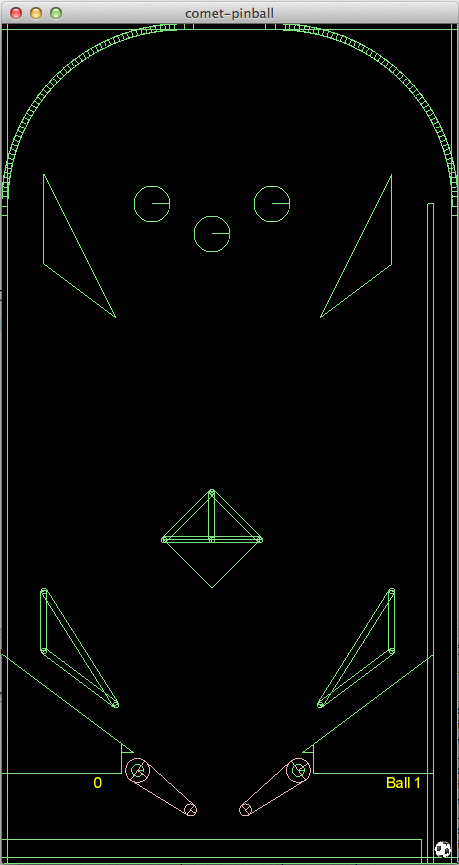
\includegraphics[height=15cm]{./img/manual/playfield.png}
	\caption[The play field]{The pinball play field when starting a new game}
	\label{fig:playfield}
\end{figure}

The play field is an inclined plane on which a ball will tend to roll downwards. An example play field can be seen in figure~\ref{fig:playfield}.

The play field has on it's right side a tube which is called a plunger tube. When bringing a new ball into play, it will be placed at the lower end of the plunger tube and can be brought into play using the plunger.

At the lower end of the field are two flippers which are used by the player to prevent the ball from passing between them into the so-called drain.

On the left side of the drain the score is displayed, on the right side the current round (ball) of play.

\subsubsection{Bumpers}

\begin{figure}
	\centering
	\begin{subfigure}[b]{0.225\textwidth}
		\centering
		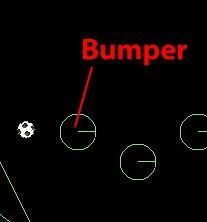
\includegraphics[width=\textwidth]{./img/manual/bumper.png}
		\caption[Bumper]{Bumper}
		\label{fig:bumper}
	\end{subfigure}
	\quad
	\begin{subfigure}[b]{0.3\textwidth}
		\centering
		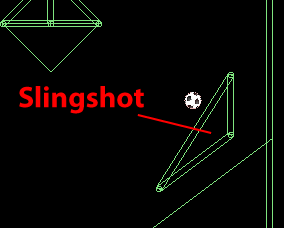
\includegraphics[width=\textwidth]{./img/manual/slingshot.png}
		\caption[Slingshot]{Slingshot}
		\label{fig:slingshot}
	\end{subfigure}
	\quad
	\begin{subfigure}[b]{0.203\textwidth}
		\centering
		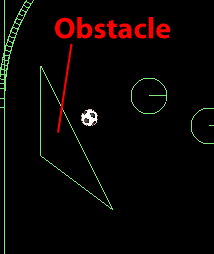
\includegraphics[width=\textwidth]{./img/manual/obstacle.png}
		\caption[Obstacle]{Obstacle}
		\label{fig:obstacle}
	\end{subfigure}
	\caption{Elements on a play field}\label{fig:elements}
\end{figure}

Bumpers are circular obstacles which react on a ball impact by applying force on the ball away from itself. Normally a player will get points for hitting a bumper as seen in figure~\ref{fig:bumper}.

\subsubsection{Slingshots}

Slingshots are obstacles with a reactive side. If the ball hits the reactive side, it is catapulted away from the slingshot. Normally a player will get points for hitting a slingshot as seen in figure~\ref{fig:slingshot}.


\subsubsection{Obstacles}

Obstacles are solid bodies on the play field which generally do not react on ball impact. The deflect the ball in its trajectory and make it harder for players to hit specific elements on the play field. An obstacle can be seen in figure~\ref{fig:obstacle}.

\subsection{Flippers}

\begin{figure}[h!]
	\centering
	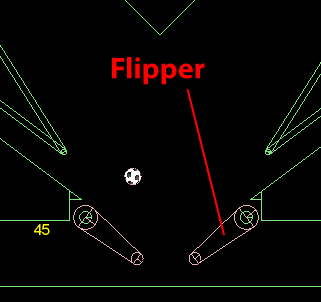
\includegraphics[height=5cm]{./img/manual/flipper.png}
	\caption[Flipper]{Flipper}
	\label{fig:flipper}
\end{figure}

Flippers bat the ball up on the play field an prevent the ball from leaving through the drain. See figure~\ref{fig:flipper}.

\section{Controls}

The game comes with a default set of controls which can be customised (see section~\ref{sec:configuration}). The following controls are used:

\begin{tabular}{ | l | l | }
\hline
\textbf{Control} & \textbf{Key} \\ \hline
Exit game & \textsc{Esc}  \\ \hline
Plunge ball & \textsc{Spacebar}  \\ \hline
Left flipper & \textsc{Tab}  \\ \hline
Right flipper & \textsc{Enter}  \\ \hline
Reset ball / End game & \textsc{R}  \\ \hline

\end{tabular}

\section{Visuals}

\subsection{Main menu}

\begin{figure}[h!]
	\centering
	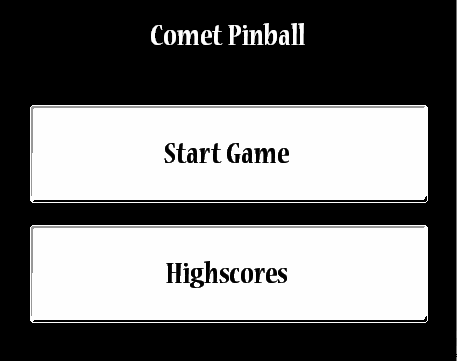
\includegraphics[height=5cm]{./img/manual/main_menu.png}
	\caption[Main menu]{Main menu}
	\label{fig:mainmenu}
\end{figure}

When starting the game the player will find himself in the main menu (figure~\ref{fig:mainmenu}). From there a new game can be started by pressing the button \emph{Start Game} or the high score can be seen by clicking on \emph{Highscores}.

\subsection{Highscores}

\begin{figure}[h!]
	\centering
	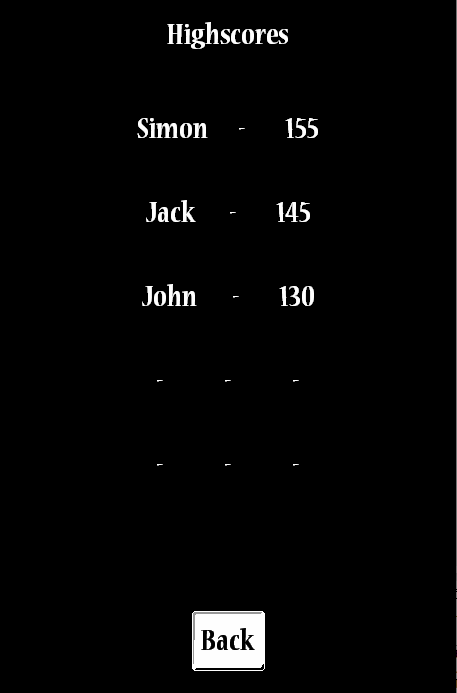
\includegraphics[height=8cm]{./img/manual/highscore.png}
	\caption[Highscores]{Highscores}
	\label{fig:highscore}
\end{figure}

On the high score screen (figure~\ref{fig:highscore}) the five best players are listed in descending order of their result. By clicking on \emph{Back} the player will get back to the main menu.

\subsection{Game over}

\begin{figure}[h!]
	\centering
	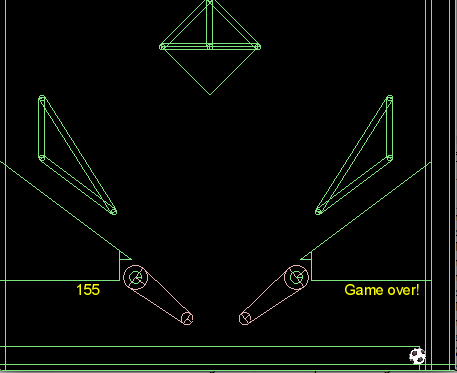
\includegraphics[height=5cm]{./img/manual/game_over.png}
	\caption[Game over]{Game over}
	\label{fig:game_over}
\end{figure}

After all balls have left the field the player is \emph{game over}, which is indicated on the play field (figure~\ref{fig:game_over}). In order to get to the next screen, the player has to press \emph{End game} (default key: \textsc{R}).

\subsection{Enter name}

\begin{figure}[h!]
	\centering
	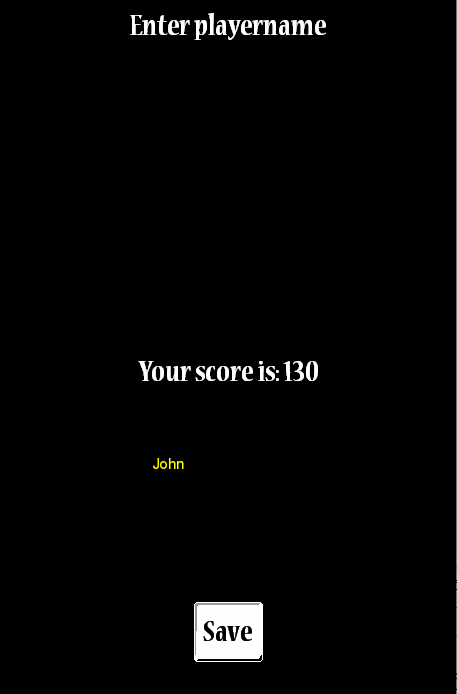
\includegraphics[height=8cm]{./img/manual/playername.png}
	\caption[Player name screen]{Player name screen}
	\label{fig:playername}
\end{figure}

After the game has ended, the player is asked to enter his name as seen on figure~\ref{fig:playername}. After having entered his name, the player should press \emph{Save} in order to save his result and get to the high score screen.

\section{Configuration}
\label{sec:configuration}

\subsection{Play field}

The playfield is configured through a file named \emph{playfields.xml} in the same folder as the game jar. If the file doesn't exist on first execution, it will be created with default content.

\begin{minipage}[]{\linewidth}
\begin{lstlisting}[language=xml,label=lst:default_playfield,caption={playfields.xml}]
<?xml version="1.0" encoding="UTF-8"?>
<configuration xmlns="http://comet.m02.ch/pinball/playfield" xmlns:xsi="http://www.w3.org/2001/XMLSchema-instance"
		xsi:schemaLocation="http://comet.m02.ch/pinball/playfield https://raw.github.com/boskoop/comet-pinball/master/schema/playfield.xsd">
	<playfields>
		<playfield>
			<name>default</name>
			<elements>
				<!-- elements -->
			</elements>
			<rules>
				<!-- rules -->
			</rules>
		</playfield>
	</playfields>
</configuration>
\end{lstlisting}
\end{minipage}

The configuration file contains a tag \texttt{playfields}, in which any number of tags of type \texttt{playfield} can be placed. Thereby it would be possible to support multiple play field configurations. At the moment this is not implemented and game will always load the first play field in the file.

A play field consists of three parts; the name, the elements and the rules. The name should be unique amongst all defined play fields in the file. The \texttt{elements} describe placable obstacles (\texttt{bumper}, \texttt{slingshot}, \texttt{obstacle}) and give them an id, which should be unique per play field. The rules assign game logic with play field elements. Using ids and a specific rule class they assign for example points for hitting an obstacle to a specific element.

The elements will be placed using absolute coordinates of the play field (origin is bottom-left, y points upwards, x to the right). The play field is 0.76 $m$ * 1.40 $m$ in size, all measures are given in meters.

\subsubsection{Bumper}

A bumper has an \texttt{id}, a \texttt{position} and a \texttt{radius}. The \texttt{id} should be unique amongst all elements, the \texttt{position} and \texttt{radius} are given in meters.

\begin{minipage}[]{\linewidth}
\begin{lstlisting}[language=xml,label=lst:bumper,caption={bumper}]
<configuration>
	<playfields>
		<playfield>
			<!-- name -->
			
			<elements>
				<bumper>
					<id>1</id>
					<position>
						<x>0.25</x>
						<y>1.1</y>
					</position>
					<radius>0.03</radius>
				</bumper>
				
				<!-- other elements -->
			</elements>
			
			<!-- rules -->
		</playfields>
	</playfield>
</configuration>
\end{lstlisting}
\end{minipage}

\subsubsection{Slingshot}

A slingshot has an \texttt{id}, a \texttt{position} and two corners, \texttt{corner.a} and \texttt{corner.b}. The \texttt{id} should be unique amongst all elements. 

\begin{figure}[h!]
	\centering
	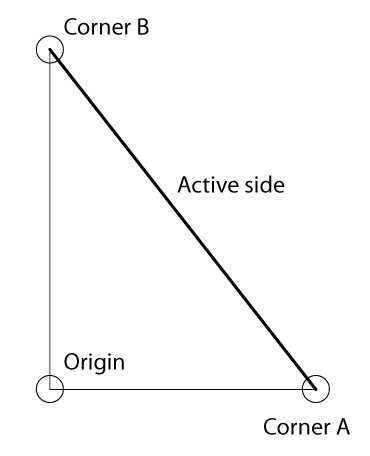
\includegraphics[height=8cm]{./img/manual/slingshot-element.png}
	\caption[Slingshot element]{Slingshot element}
	\label{fig:slingshot_element}
\end{figure}

Figure~\ref{fig:slingshot_element} pictures how a slingshot is defined. The origin is given by the \texttt{position} of the element, \texttt{corner.a} and \texttt{corner.b} are defined using a vector (x/y) relative to the origin.

\textbf{\textsl{Important:}} The corners origin, a and b must always form a triangle in \textsl{anticlockwise} direction, or the element will not be simulated correctly!

\begin{minipage}[]{\linewidth}
\begin{lstlisting}[language=xml,label=lst:slingshot,caption={slingshot}]
<configuration>
	<playfields>
		<playfield>
			<!-- name -->
			
			<elements>
				<slingshot>
					<id>5</id>
					<position>
						<x>0.65</x>
						<y>0.355</y>
					</position>
					<corner.a>
						<x>0.0</x>
						<y>0.1</y>
					</corner.a>
					<corner.b>
						<x>-0.12</x>
						<y>-0.09</y>
					</corner.b>
				</slingshot>
				
				<!-- other elements -->
			</elements>
			
			<!-- rules -->
		</playfields>
	</playfield>
</configuration>
\end{lstlisting}
\end{minipage}

\subsubsection{Obstacle}

An obstacle has an \texttt{id}, a \texttt{position} and a list of \texttt{vertices} The \texttt{id} should be unique amongst all elements. 

\begin{figure}[h!]
	\centering
	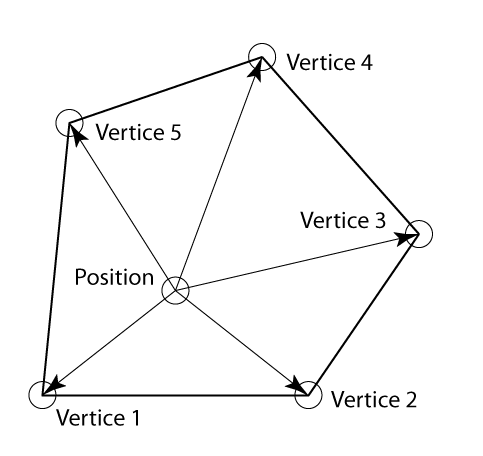
\includegraphics[height=8cm]{./img/manual/obstacle-element.png}
	\caption[Obstacle element]{Obstacle element}
	\label{fig:obstacle_element}
\end{figure}

Figure~\ref{fig:obstacle_element} pictures how an obstacle is defined. The \texttt{position} is given by absolute coordinates on the play field. Every \texttt{vertice} defines a point in relative coordinates to the \texttt{position} where a corner should be. The \texttt{position} itself can be a corner too, if there is a $(0/0)$ \texttt{vertice}.

\textbf{\textsl{Important:}} The \texttt{vertices} must always form a \textsl{convex} polygon with corners in \textsl{anticlockwise} direction, or the element will not be simulated correctly! The number of vertices is limited to 8 per obstacle.

\begin{minipage}[]{\linewidth}
\begin{lstlisting}[language=xml,label=lst:obstacle,caption={obstacle}]
<configuration>
	<playfields>
		<playfield>
			<!-- name -->
			
			<elements>
				<obstacle>
					<id>6</id>
					<position>
						<x>0.65</x>
						<y>1.0</y>
					</position>
					<vertices>
						<vertice>
							<x>0.0</x>
							<y>0.0</y>
						</vertice>
						<vertice>
							<x>0.0</x>
							<y>0.15</y>
						</vertice>
						<vertice>
							<x>-0.12</x>
							<y>-0.09</y>
						</vertice>
					</vertices>
				</obstacle>
				
				<!-- other elements -->
			</elements>
			
			<!-- rules -->
		</playfields>
	</playfield>
</configuration>
\end{lstlisting}
\end{minipage}

\subsubsection{Rules}

\texttt{Rules} define logic on a play field. A play field can have an arbitrary amount of \texttt{rules} defined. Every \texttt{rule} consists of a rule \texttt{class} and a list of \texttt{parameters}. The rule \texttt{class} must be defined using its fully qualified class name. The number of \texttt{parameters} is defined by the \texttt{rule} itself.

At the moment there is only the \texttt{rule} \emph{HitScoreRule} implemented, which takes two parameters, an id of the affected element an the number of points the player gets, when the ball hits the element.

\begin{minipage}[]{\linewidth}
\begin{lstlisting}[language=xml,label=lst:rule,caption={rule}]
<configuration>
	<playfields>
		<playfield>
			<!-- name -->
			<!-- elements -->
			
			<rules>
				<rule>
					<class>ch.m02.comet.pinball.logic.simulation.rule.basic.HitScoreRule</class>
					<parameters>
						<parameter>1</parameter>
						<parameter>20</parameter>
					</parameters>
				</rule>
				
				<!-- other rules -->
			</rules>
		</playfields>
	</playfield>
</configuration>
\end{lstlisting}
\end{minipage}

\subsection{Reset stats}

On first execution, the game will create a file named \emph{pinball.ser} which contains persistent information about played games. In order to reset all statistics the file can be deleted.

\subsection{Properties}

In the root of the game jar, there is a configuration file \emph{pinball.properties} located. Using these properties, the pinball game can be configured.

\begin{minipage}[]{\linewidth}
\begin{lstlisting}[label=lst:properties,caption={pinball.properties}]
pinball.debug=false
pinball.skip.splashscreen=false

# Keys
key.game.exit=ESCAPE
key.ball.up=UP
key.ball.left=LEFT
key.ball.right=RIGHT
key.ball.plunge=SPACE
key.ball.reset=R
key.flipper.left=TAB
key.flipper.right=ENTER

# Physics
physics.pinball.radius=0.0135
physics.earth.gravity=-9.81
physics.ramp.angle.degrees=7.0
\end{lstlisting}
\end{minipage}

\subsubsection{pinball.debug}

This property enables some more extensive logging and manipulation of the ball using the arrow keys.

\subsubsection{pinball.skip.splashscreen}

Enables/disables the splash screen.

\subsubsection{key.*}

Configures the keys for user interaction.

\subsubsection{physics.*}

Sets physics values, the units are in $m$, $m/s^{2}$ and degrees.

\end{document}
